\documentclass[../main.tex]{subfiles}

\begin{document}

\chapter{Network analysis of cell-cell connectivity}
\label{cha:networking}


\begin{figure}[ht]
  \centering
  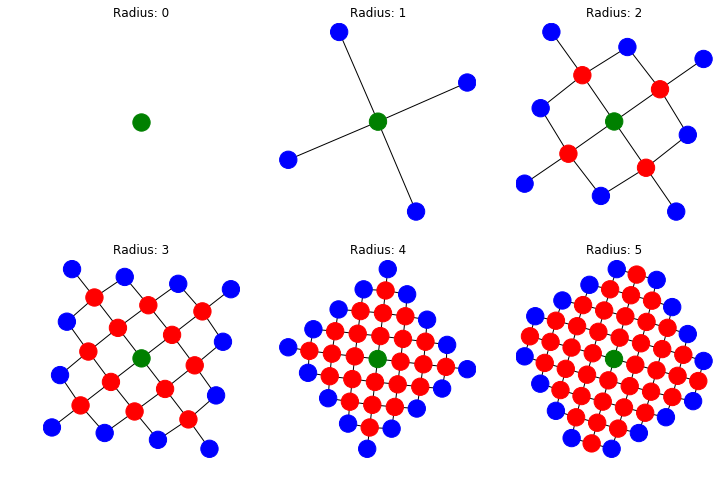
\includegraphics[width=\columnwidth]{figures/radius illustration.png}
  \caption{\label{fig:radiusconnectivity}Radius connections}
\end{figure}


\begin{figure}[!ht]
  \centering
     \subfloat[First sub-figure\label{subfig-1:connectivity}]{%
       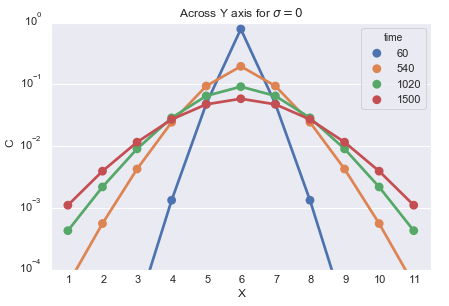
\includegraphics[width=0.4\columnwidth]{./figures/conn1.png}
     }
     \subfloat[First sub-figure\label{subfig-2:connectivity}]{%
       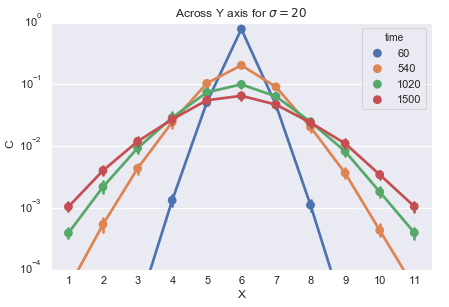
\includegraphics[width=0.4\columnwidth]{./figures/conn2.png}
     }
     \\
     \subfloat[First sub-figure\label{subfig-3:connectivity}]{%
       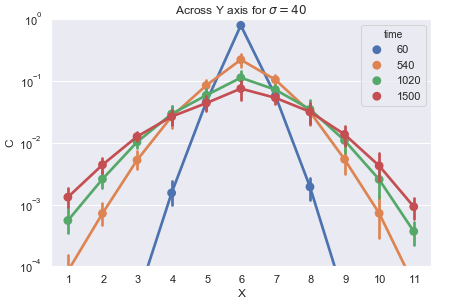
\includegraphics[width=0.4\columnwidth]{./figures/conn3.png}
     }
     \subfloat[First sub-figure\label{subfig-3:connectivity}]{%
       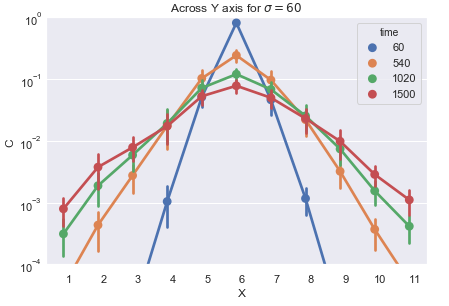
\includegraphics[width=0.4\columnwidth]{./figures/conn4.png}
     }
     \caption{Connectivity}
     \label{fig:connectivity}
   \end{figure}


\section{Images to networks}
\label{sec:img2network}

   


\begin{figure}[!ht]
  \centering
  \subfloat[First sub-figure\label{subfig-1:img2networks}]{%
    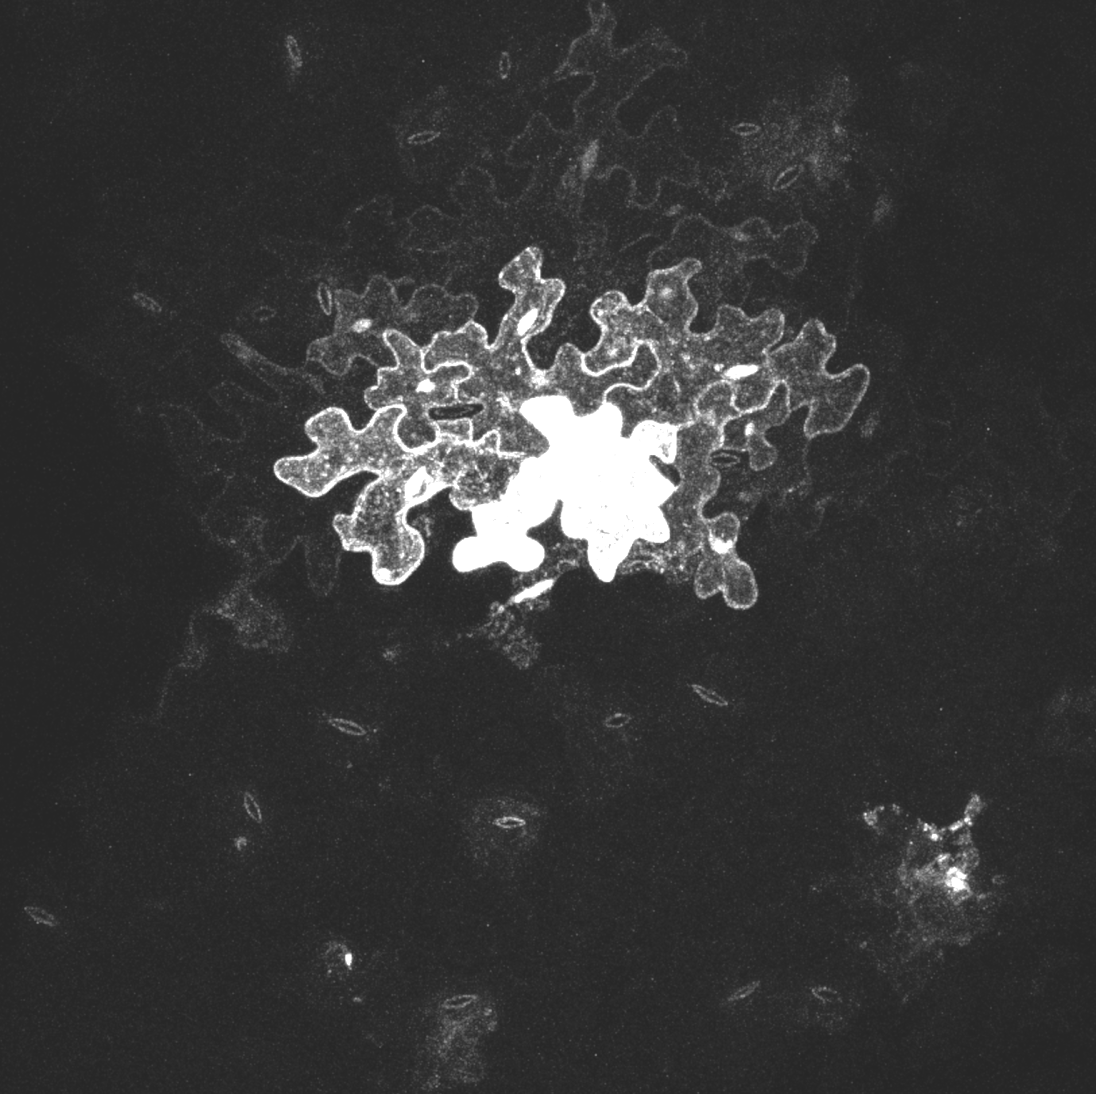
\includegraphics[width=0.4\columnwidth]{./figures/orig.png}
  }
  \subfloat[First sub-figure\label{subfig-2:img2networks}]{%
    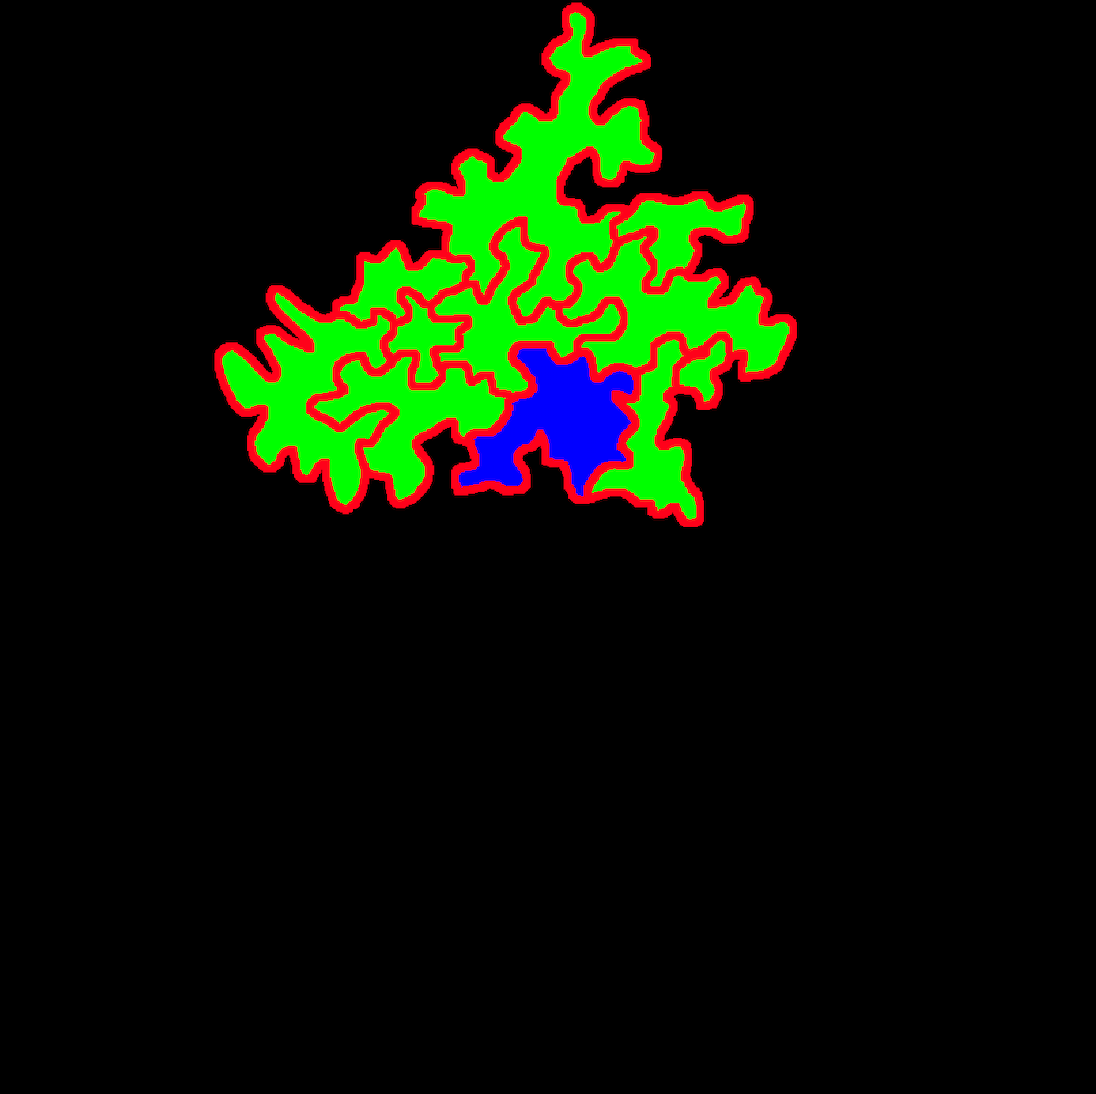
\includegraphics[width=0.4\columnwidth]{./figures/step1.png}
  }
  \\
  \subfloat[First sub-figure\label{subfig-3:img2networks}]{%
    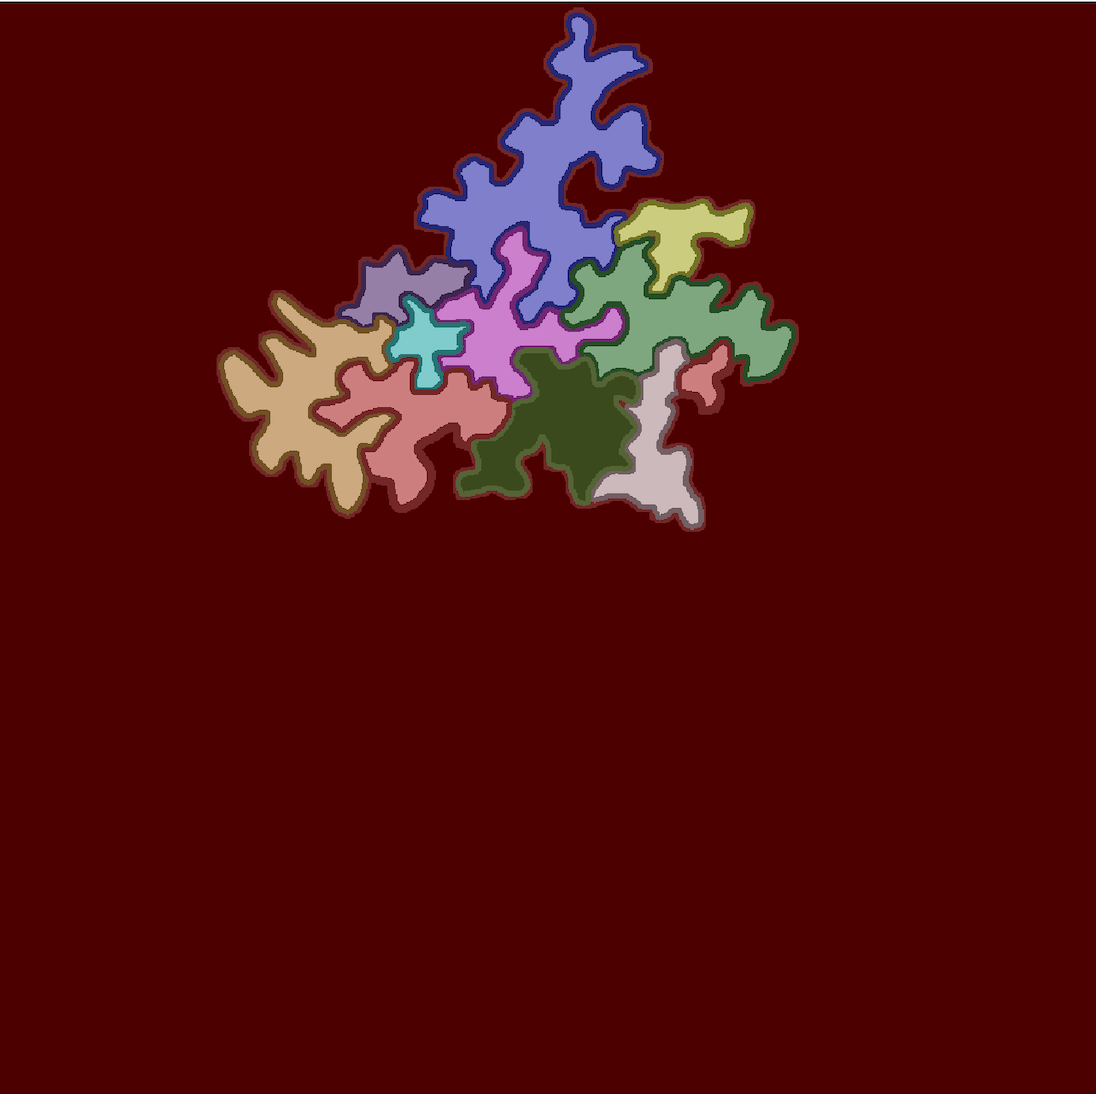
\includegraphics[width=0.4\columnwidth]{./figures/step2.png}
  }
  \subfloat[First sub-figure\label{subfig-3:img2networks}]{%
    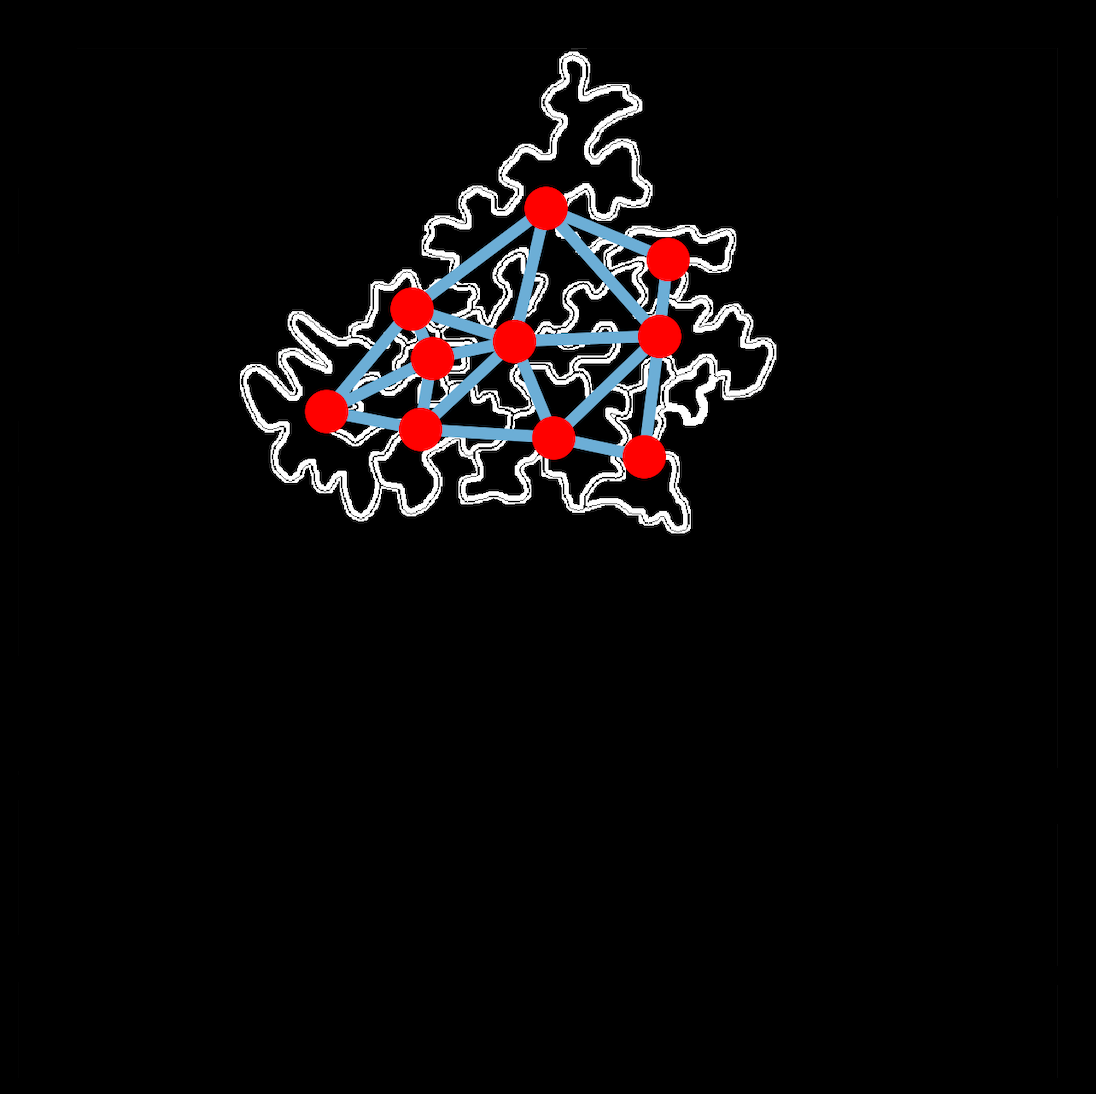
\includegraphics[width=0.4\columnwidth]{./figures/step3.png}
  }
  \caption{Connectivity}
  \label{fig:img2networks}
\end{figure}







\end{document}


%%% Local Variables:
%%% mode: latex
%%% TeX-master: "../main"
%%% End:
